\section{Additional Empirical Figures}
\label{app:additional-figures}

The main text keeps only the figures needed for the core narrative. This appendix retains supporting diagnostics that are useful for auditability but would distract from the main flow.

% \begin{figure}[p]
% \centering
% 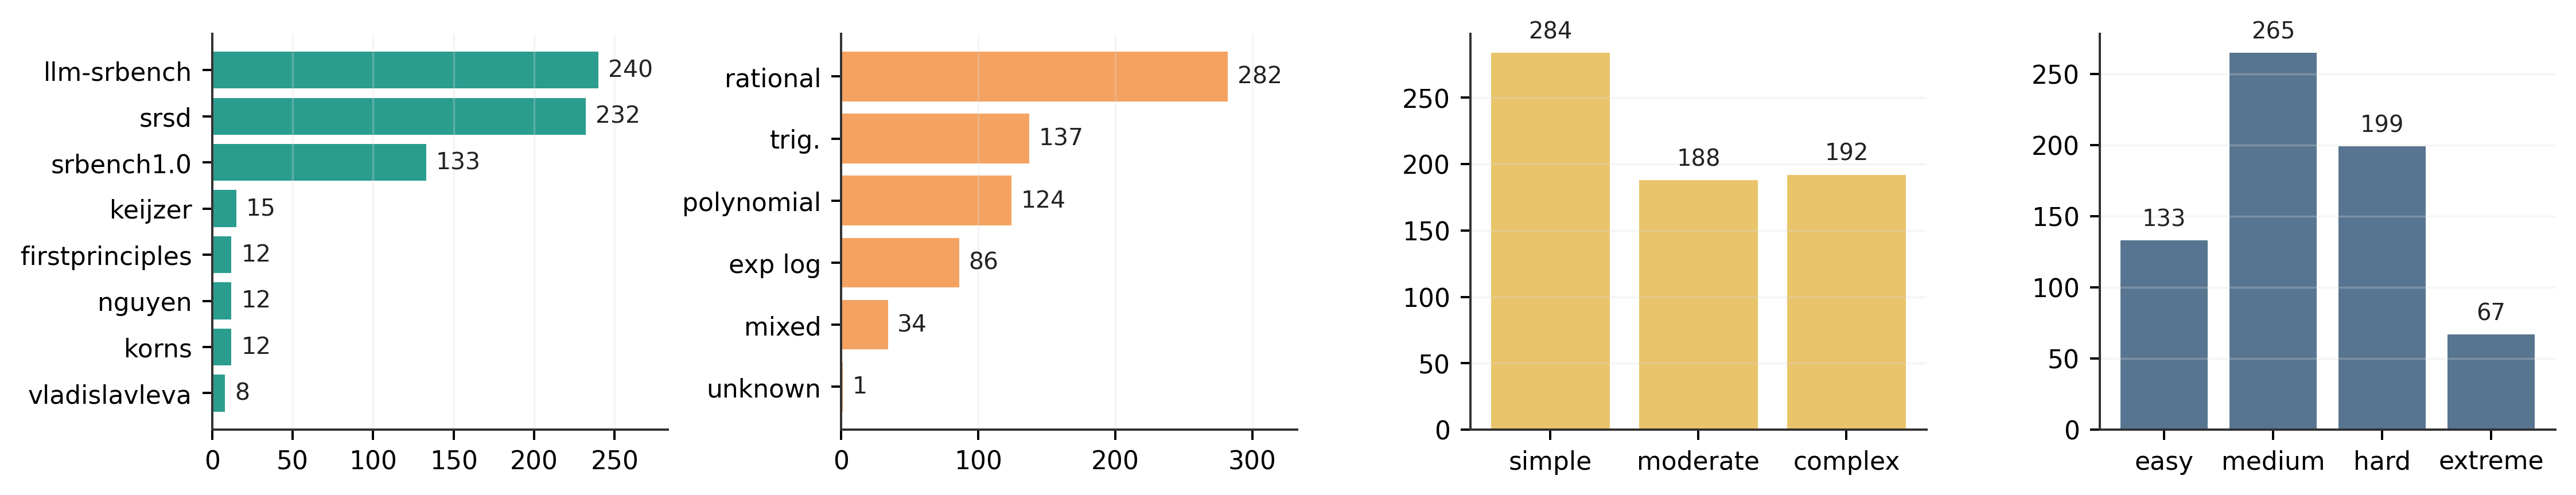
\includegraphics[width=0.88\linewidth]{imgs/Article/figure02_reservoir_composition}
% \caption{\reservoir{} composition after ground-truth filtering. The reservoir retains heterogeneous source families, operator profiles, formula complexities, and probe-derived difficulty bins; this is why later selection must control both static metadata and response-derived behavior.}
% \label{fig:appendix-reservoir-composition}
% \end{figure}

\begin{figure}[p]
\centering
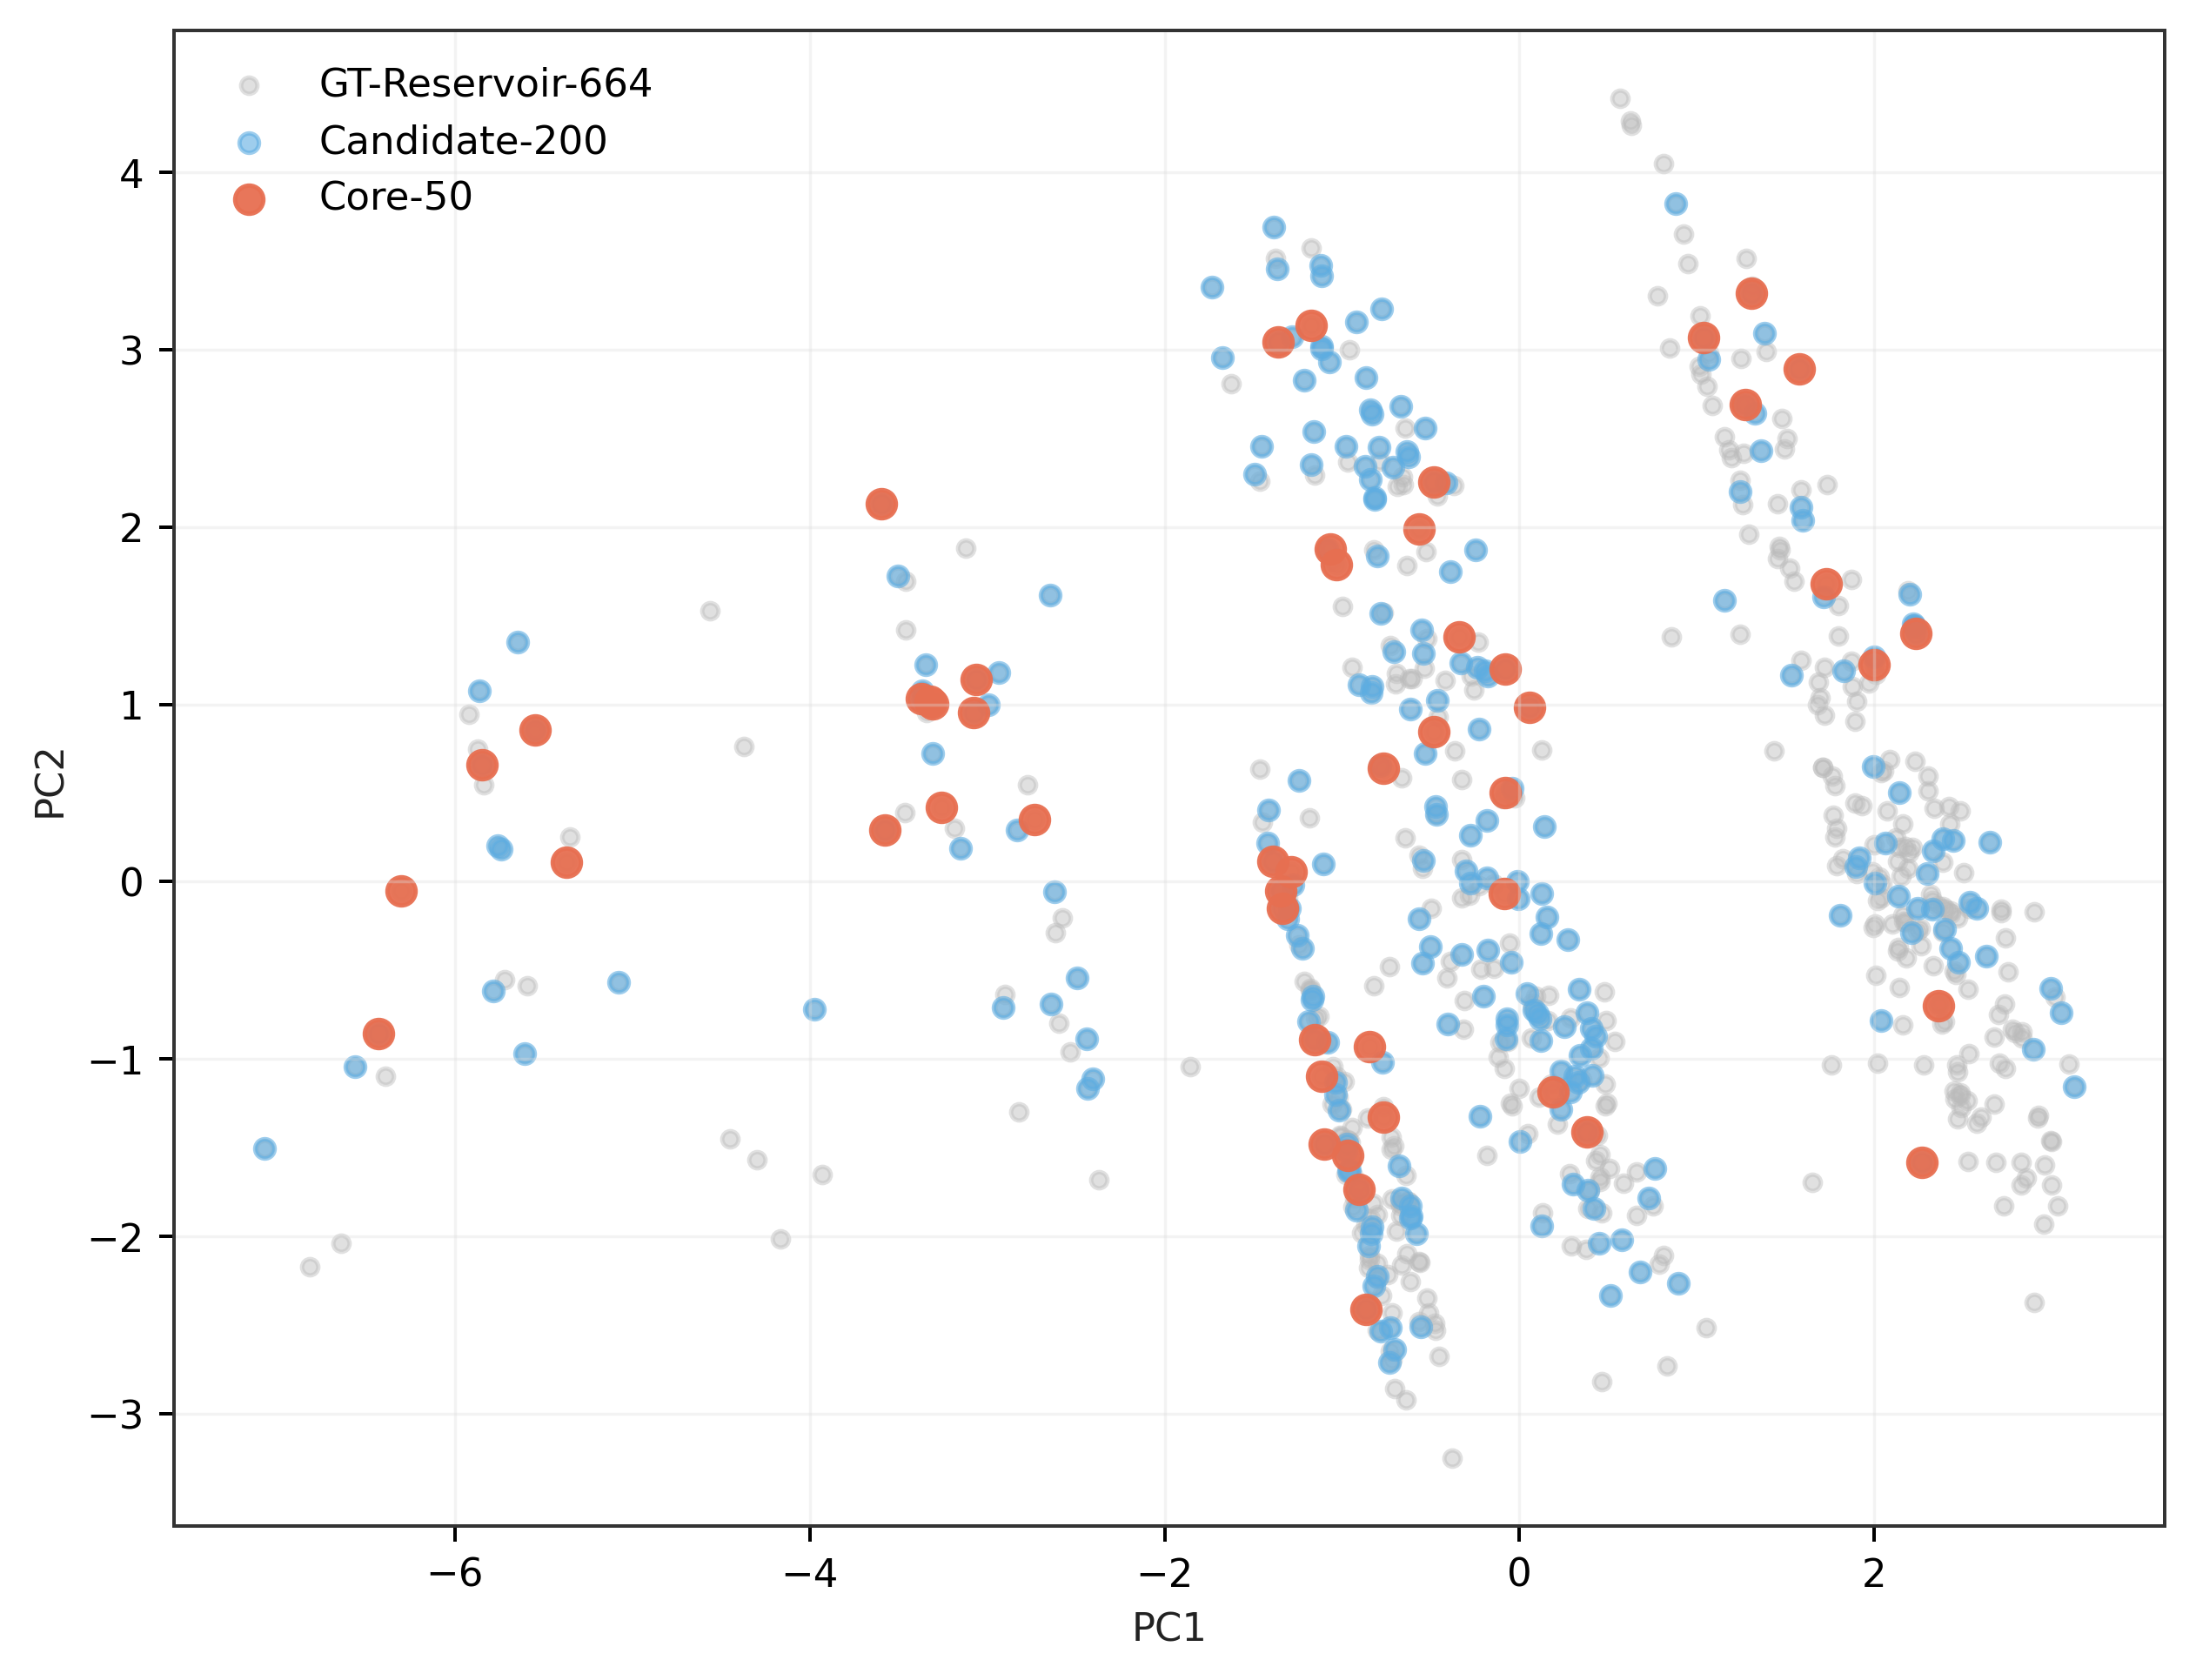
\includegraphics[width=0.82\linewidth]{imgs/Article/figure10_core50_coverage_map}
\caption{\textbf{\core{} coverage over \reservoir{}.} \core{} coverage over the reservoir-derived structural and Probe-4 response profile. The selected subset remains compact, but it covers the main family, difficulty, failure-mode, and response-pattern regions rather than collapsing into a single high-gap corner.}
\label{fig:appendix-core50-coverage-map}
\end{figure}

\begin{figure}[p]
\centering
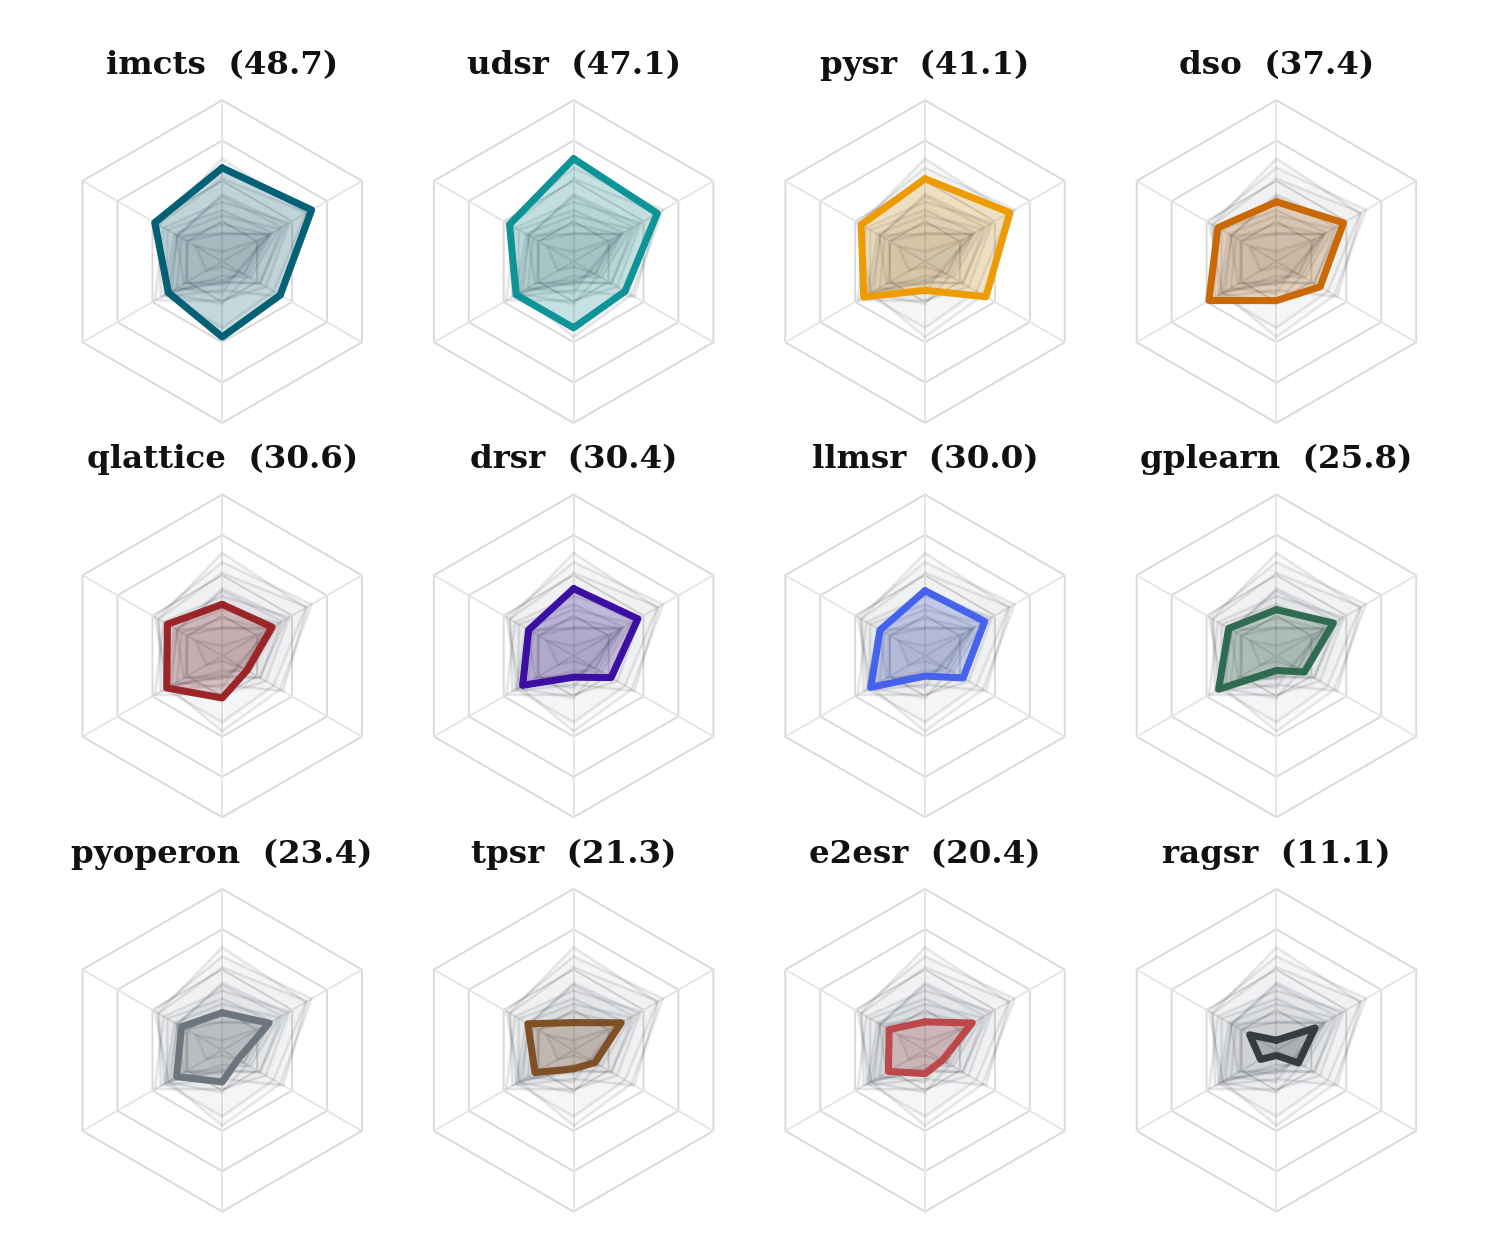
\includegraphics[width=0.86\linewidth]{imgs/Article/fig_hexagon_small_multiples_neurips}
\caption{\textbf{Per-algorithm clean-track profiles.} The small multiples make the same point as the main heatmap at algorithm level: similar OOD rankings can still hide differences in symbolic fidelity, efficiency, and effective stability.}
\label{fig:appendix-hexagon-small-multiples}
\end{figure}

\begin{figure}[p]
\centering
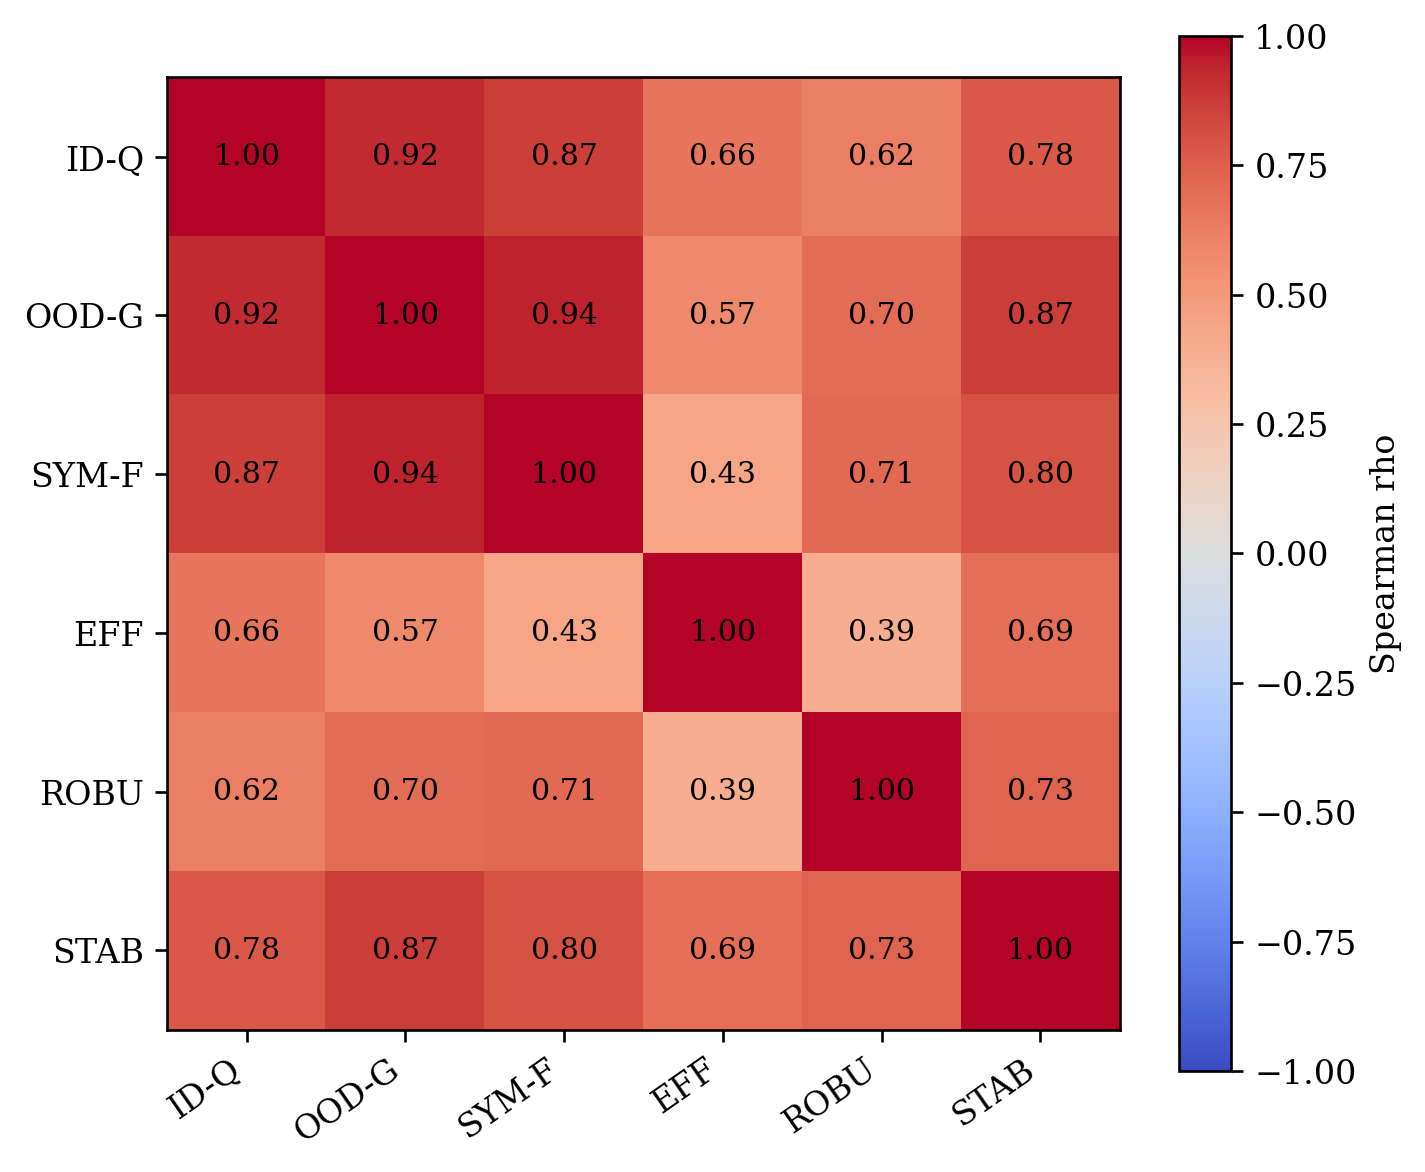
\includegraphics[width=0.76\linewidth]{imgs/Article/figure29_axis_correlation_matrix}
\caption{\textbf{Clean-track axis correlation structure.} The axes and robustness extension are related, but they do not collapse into a single numerical-error score, motivating separate reporting rather than one opaque aggregate.}
\label{fig:appendix-axis-correlation}
\end{figure}

\begin{figure}[p]
\centering
\begin{minipage}{0.48\linewidth}
\centering
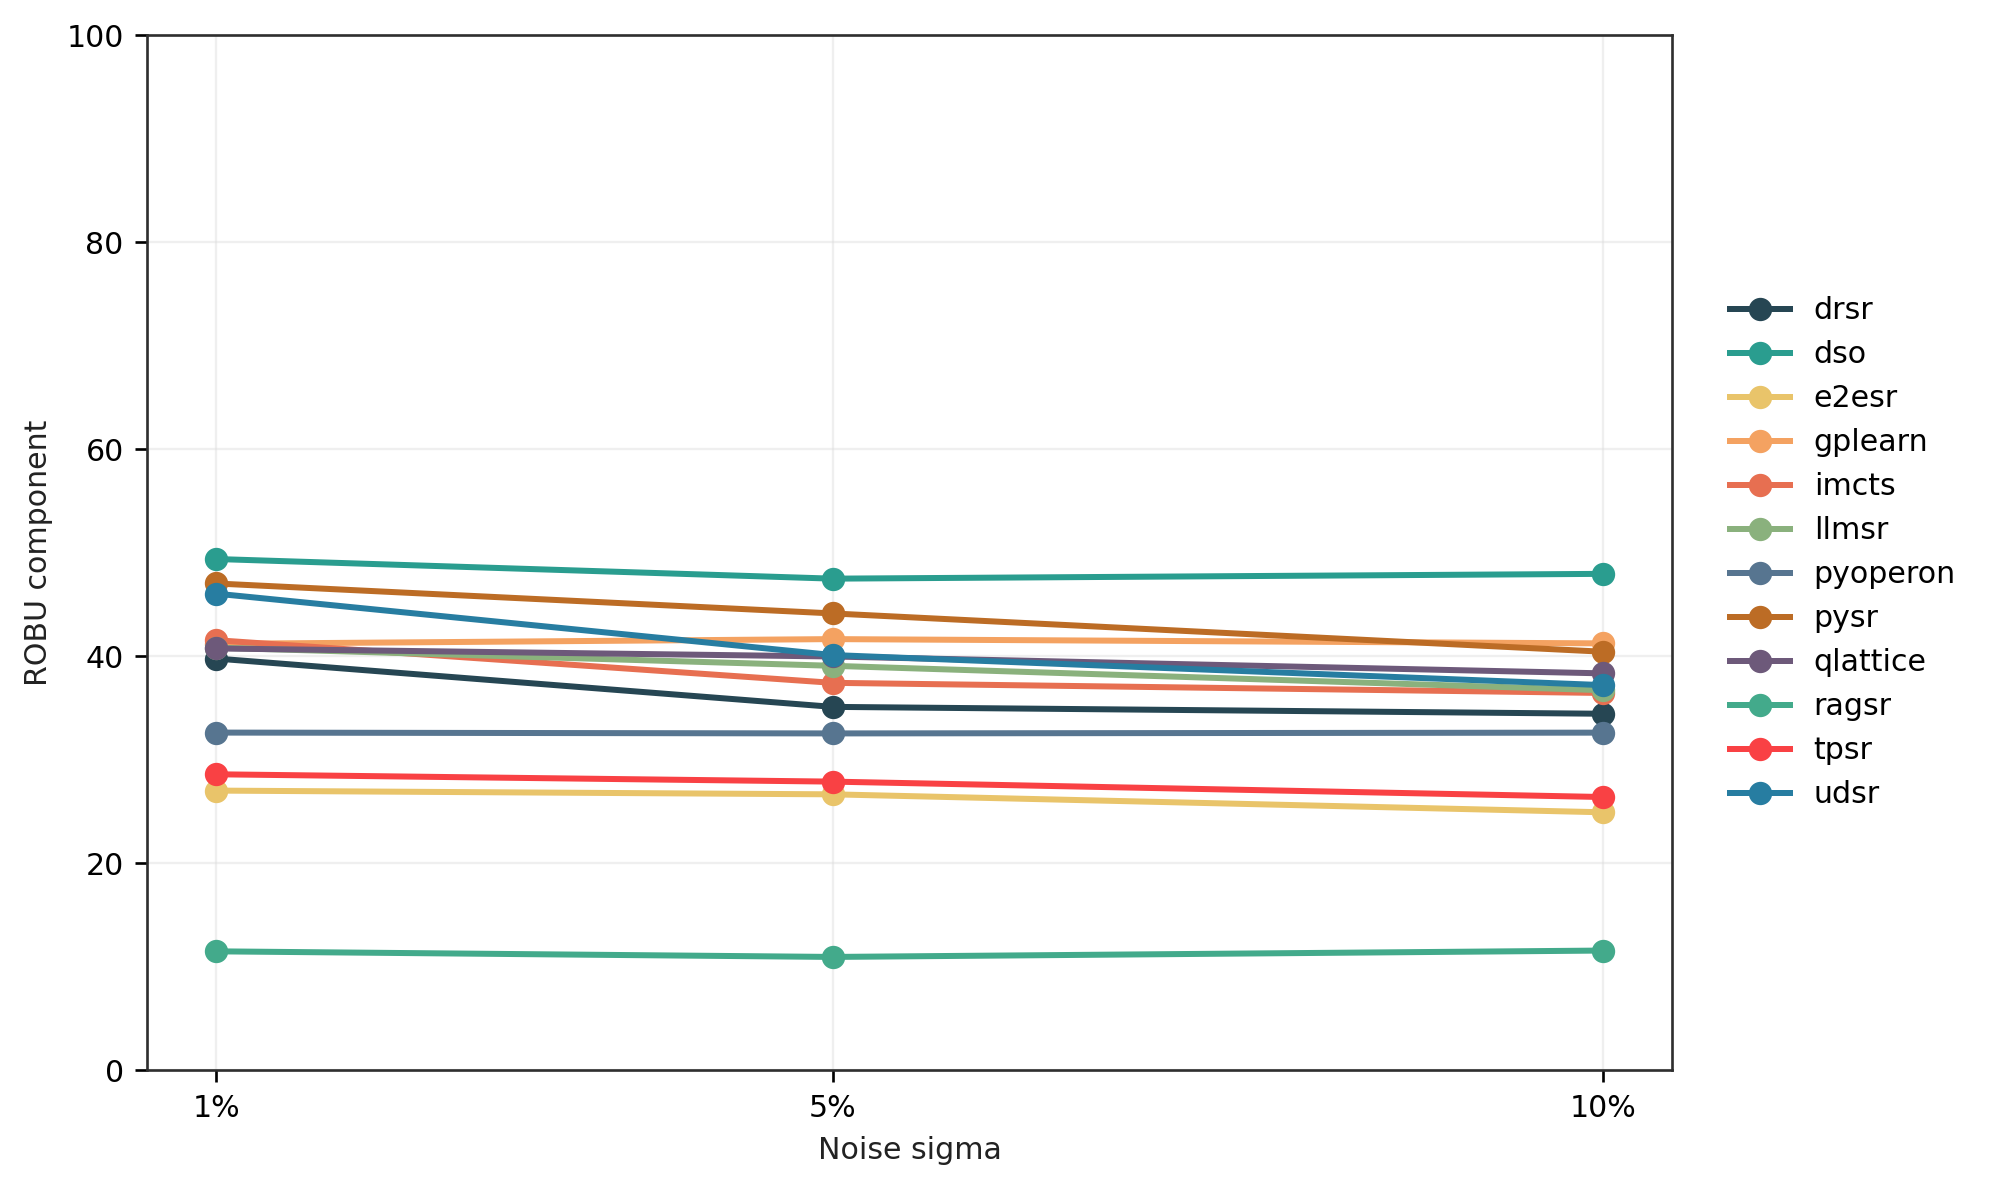
\includegraphics[width=\linewidth]{imgs/Article/figure25_noise_robustness_curve}
\end{minipage}
\hfill
\begin{minipage}{0.48\linewidth}
\centering
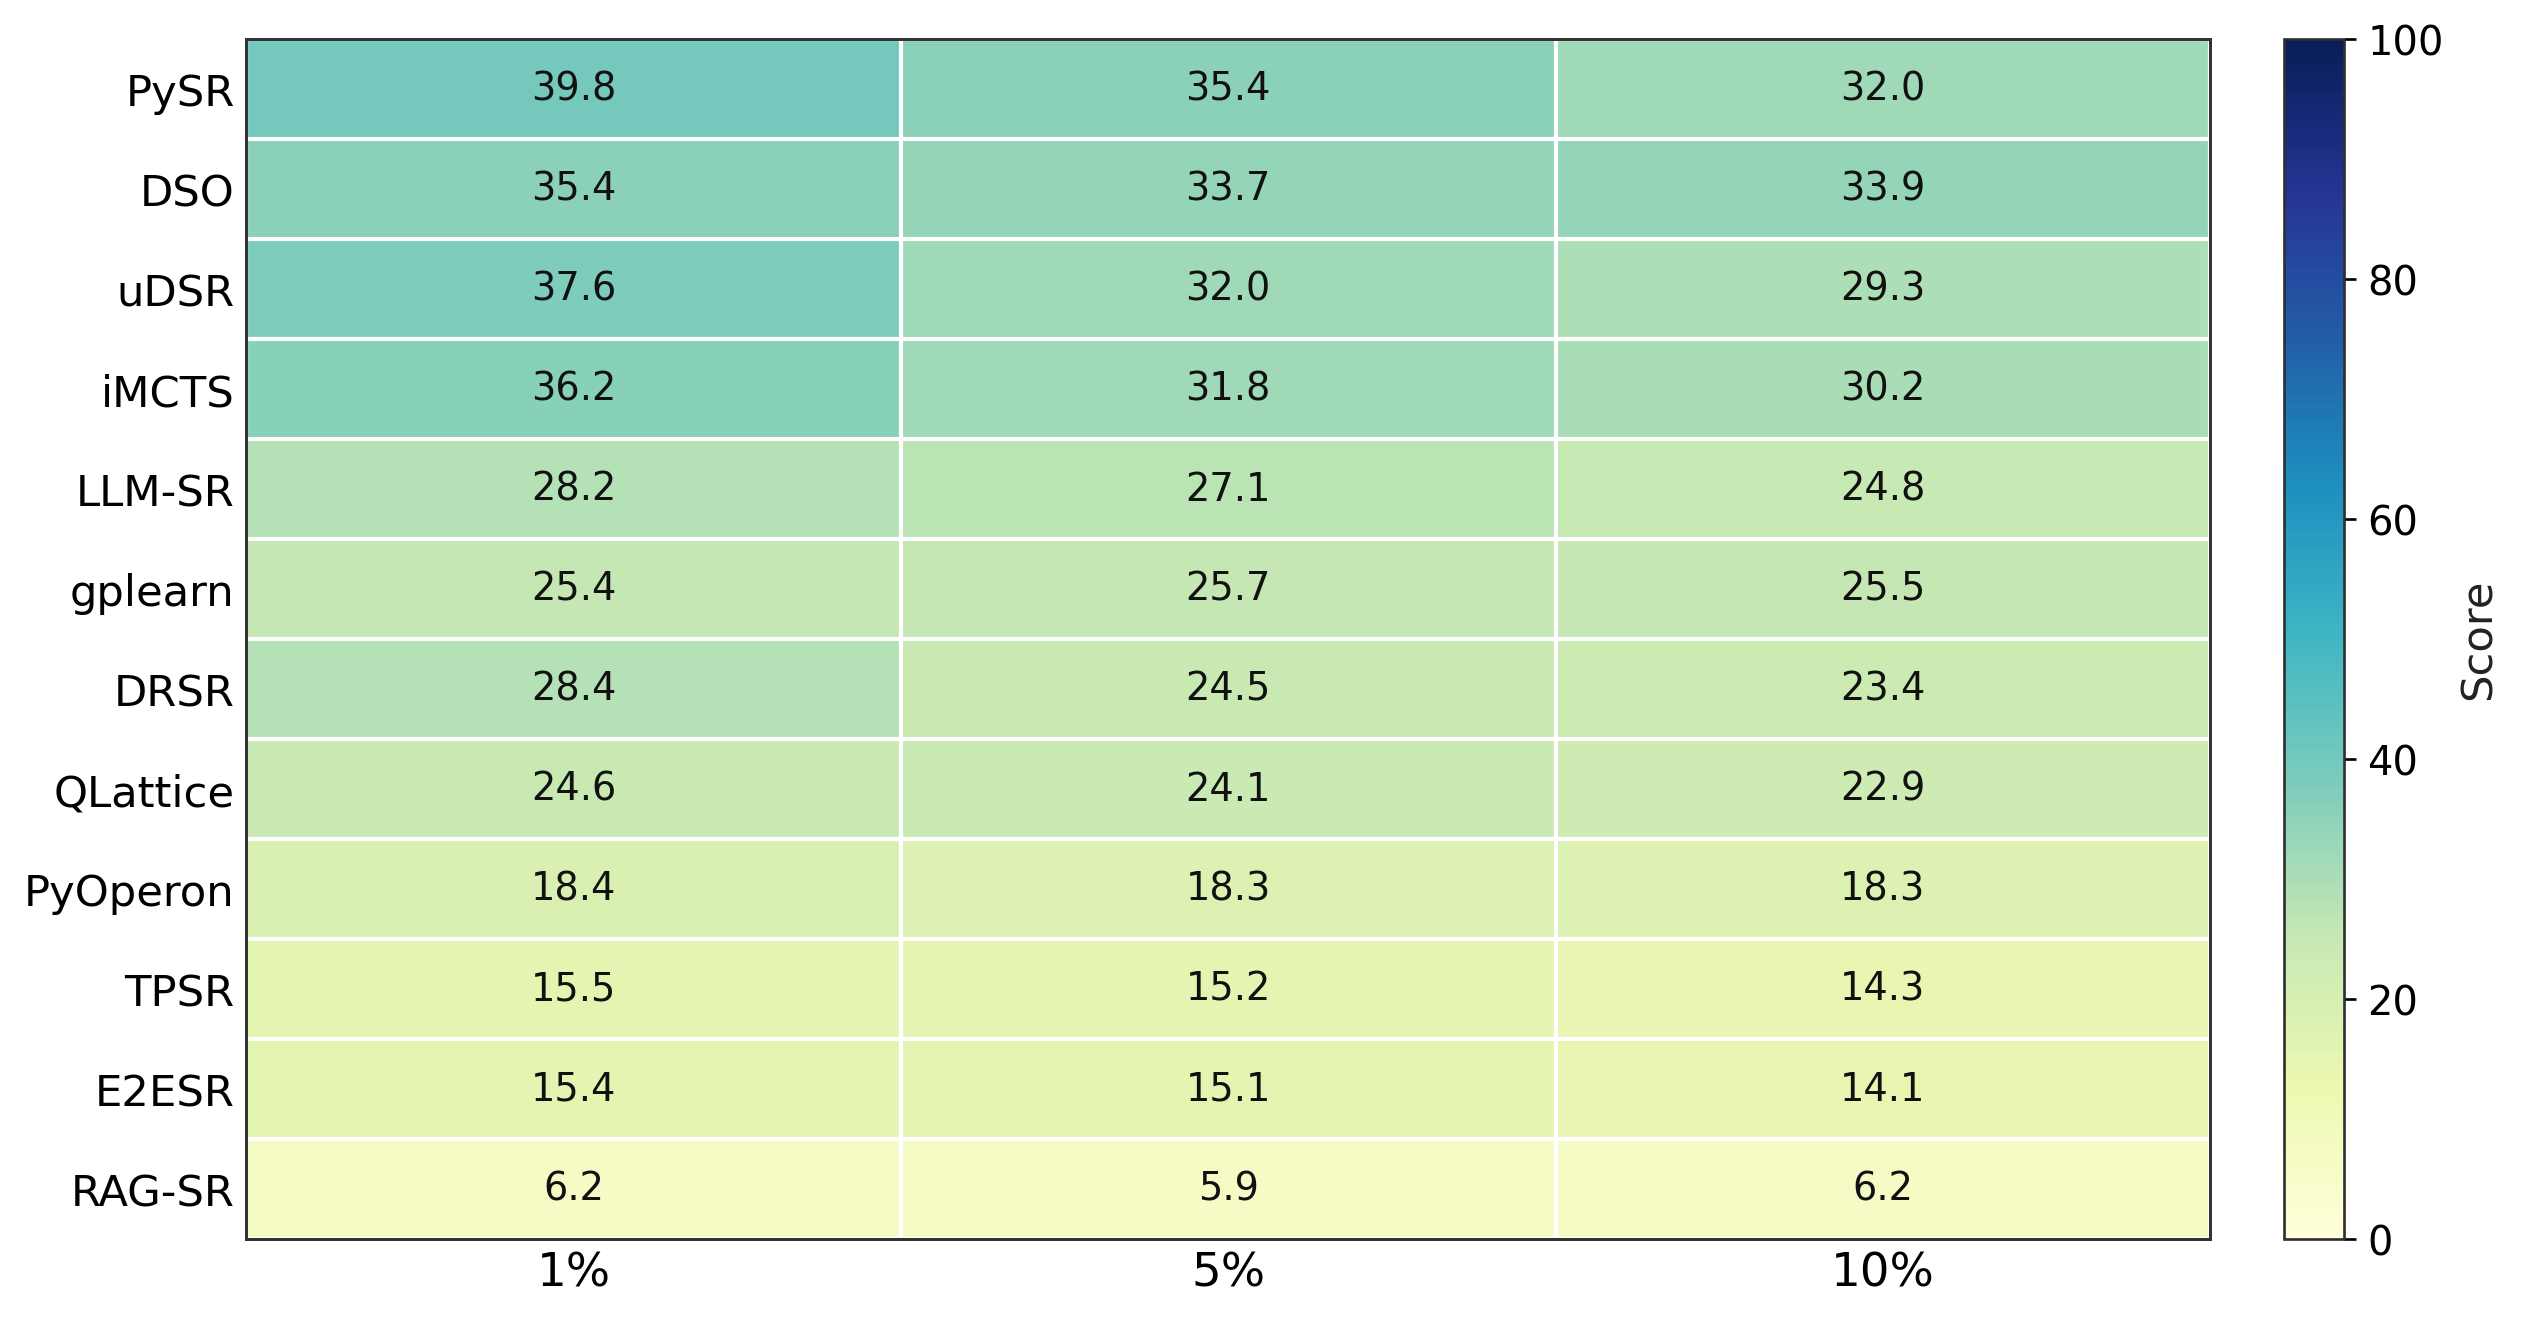
\includegraphics[width=\linewidth]{imgs/Article/figure26_noise_quality_heatmap}
\end{minipage}
\caption{\textbf{Noisy-training robustness extension.} Left: robustness curves summarize clean-test quality under increasing training noise. Right: the noise-quality heatmap shows which algorithms retain usable formulas under the standardized noisy-track protocol.}
\label{fig:appendix-robustness-extension}
\end{figure}
